%%%%%%%%%%%%%%%%%%%%%%%%%%%%%%%%%%%%%%%%%%%%%%%%%%%%%%%%%%%%%%%%%%%%%
%% Start the main part of the manuscript here.
%%%%%%%%%%%%%%%%%%%%%%%%%%%%%%%%%%%%%%%%%%%%%%%%%%%%%%%%%%%%%%%%%%%%%
\section{Introduction}

Protein-protein interface interactions underly many biological processes, including control of complex systems and antibody-antigen recognition.
In fact, mutations at protein-protein interfaces are over-represented within disease-causing mutations\cite{jubb_mutations_2017}, indicating the central importance of these interactions to biology and impications to human health.
An ability to computationally predict the strength of and perturb these interactions would not only serve as a useful experimental tool to improve our understanding of biology, but would also enhance our ability to create drugs with novel methods of actions, and additionally enhance engineering applications such as design of protein biosensors.
In particular, as there are over 9500 known domain-domain interactions in the PDB \cite{finn_ipfam:_2014}, a computational method capable of predicting mutations that strengthen or weaken known protein-protein interactions would provide a tool capable of precisely perturbing these interactions in such a way to generate knowledge about biological processes or improve drug function.


Prior methods have attempted to predict changes in binding free energies by taking various approaches,
including using weighted energy functions that set to describe physical interactions underlying protein-protein interactions\cite{guerois_predicting_2002,kamisetty_accounting_2011},
statistical and contact potentials \cite{dehouck_beatmusic:_2013,moal_intermolecular_2013,vangone_contacts-based_2015,brender_prediction_2015},
a combination of these approaches\cite{li_predicting_2014},
graph-based representations\cite{pires_mcsm:_2014},
methods focused on antibodies\cite{lippow_computational_2007},
and methods that attempt to sample backbone structure space locally around mutations\cite{dourado_multiscale_2014}.

We set out to create a method for prediction of change in binding free energy after mutation (interface \ddg) within the Rosetta macromolecular modeling suite, which is freely available for academic usage, allowing future combination of these predictions with Rosetta's powerful protein design capabilities, which has proven successful in a variety of applications \cite{tinberg_computational_2013,kaufmann_practically_2010}.
Prior projects have studied the applied ability of Rosetta specifically to enhance protein-protein binding affinities \cite{sammond_structure-based_2007} and to design influenza inhibitors \cite{whitehead_optimization_2012}, but no prior benchmarking effort has studied the performance of change in binding free energy predictions in Rosetta on a large, diverse benchmark data set, in part because such a dataset has only become available more recently.
The preexisting state-of-the-art Rosetta \ddg\ method,  ddg\_monomer \cite{kellogg_role_2011}, has been proven effective at predicting changes in stability in monomeric proteins after mutation, but had not yet been tested at predicting change of binding free energies in protein-protein complexes.
Prior ``alanine scanning'' \ddg\ methods were benchmarked in interfaces, but only for mutations for alanine \cite{kortemme_simple_2002,kortemme_computational_2004,conchuir_web_2015}.
These alanine scanning methods sampled only side chain degrees of freedom, which is a fair approximation to make for mutations to alanine (which are not expected to cause large backbone perturbations\cite{cunningham_high-resolution_1989}), but a less probable assumption for mutations to larger side chains, as some degree of backbone rearrangement is expected to be necessary to accomodate these larger mutations.
Adaptation of these alanine scanning methods to recent score function and sampling methods has not shown improvement in benchmarking\cite{conchuir_web_2015}, indicating a need to more thoroughly develop and test a method that attempts to more aggressively sample conformational space.

We sought to create a method that would take into account the natural conformational flexibility and dynamics of proteins by representing structures as an ensemble of individual full-atom models, generating sufficient microstate-like models to effectively cover the biologically relevant and and accessible portions of the free energy landscape.
Ensemble representations have proven their effectiveness to predict change in protein stabilities after mutation\cite{benedix_predicting_2009} and to improve $\Delta G_{binding}$ calculations between kinases and their inhibitors \cite{araki_effect_2016}.

We chose to sample conformational diversity through use of the ``backrub'' protocol implemented in Rosetta.
The backrub method samples using local, coupled, side chain and backbone motions, similar to those observed in high-resolution crystal structures \cite{davis_backrub_2006}.
Backrub ensembles appears to recapitulate properties of proteins that have been experimentally determined, such as side chain NMR order parameters\cite{friedland_simple_2008}, sequence profiles at protein-protein interfaces \cite{humphris_prediction_2008}, sequence profiles of protein-peptide binding specificity \cite{smith_structure-based_2010,smith_predicting_2011}, and can sample the conformational variability between protein homologs\cite{schenkelberg_protein_2016}.
Backrub has also proved effective in design applications, such as for the redesign of ligand-binding specificity\cite{ollikainen_coupling_2015}.
When Davey and Chica compared backrub ensembles to ensembles generated via molecular dynamics simulations or PertMin, backrub ensembles were shown in certain cases to be
``the only ensemble which has a diversity that is greater than its average deviation from crystal structure, a consequence of the ability of Backrub motions to mimic high resolution dynamics from solution NMR while maintaining structural similarity to the input crystal structure''.\cite{davey_improving_2014}
We hypothesized that this property of backrub ensembles would translate into these ensembles serving as an effective structural representation to use when predicting interface \ddg\ values.

\section{Methods}

Developing and testing with confidence a new method to predict changes in binding free energy after mutation requires a large benchmark set of covering single mutations, multiple mutations, mutations to all amino acid types, and mutations across a variety of complexes.
Skempi \cite{moal_skempi:_2012} is the largest known database of known \ddg s in protein-protein interfaces, but can be curated further for maximum effectiveness for method development and benchmarking.
In part to prevent overfitting our method on a benchmark set of our own creation, we have chosen to use a dataset created by Dourado and Flores\cite{dourado_multiscale_2014} during the creation of their ZEMu (Zone Equilibration of Mutants) method.
The ZEMu dataset was curated for effectiveness in benchmarking an interface \ddg\ method, including filtering SKEMPI values derived from non-peer reviewed data.
Confidence in the ``known'' experimental \ddg\ values is important, as it has been shown that the experimental methodology used can have a strong effect on the performance of predictors of changes in binding free energy\cite{geng_exploring_2016}.
The ZEMu dataset was also curated to include a wide range of both stabilizing and destabilizing mutants, small side chain to large side chain mutations, single and multiple mutations, and a diversity of complexes (\cref{tab:table-composition}).

\subimport*{figs-and-tables/}{table-composition}

After a review of the literature from which the known experimental \ddg\ values originated from, we removed one data point from the 1254 point ZEMu set that we could not match to the originally published reported affinity value. We also removed 5 mutations we determined to be duplicates, along with 8 mutations that were reverse mutations of other data points, leaving us with a test set of 1240 mutations.
We defined which complexes that contained at least one antibody binding partner by comparison of PDB identifiers with SAbDab \cite{dunbar_sabdab:_2014}.

We have implemented our flex ddG protocol within the RosettaScripts scripting interface to the Rosetta macromolecular modeling software suite \cite{fleishman_rosettascripts:_2011}, which makes the protocol easily adaptable to future improvements and energy function development. We utilized the Talaris \cite{leaver-fay_chapter_2013,song_structure-guided_2011,shapovalov_smoothed_2011} and Ref\cite{alford_rosetta_2017} energy functions in Rosetta. Version numbers of tested software are available in \cref{tab:table-versions}.

\begin{figure}
  \centering
  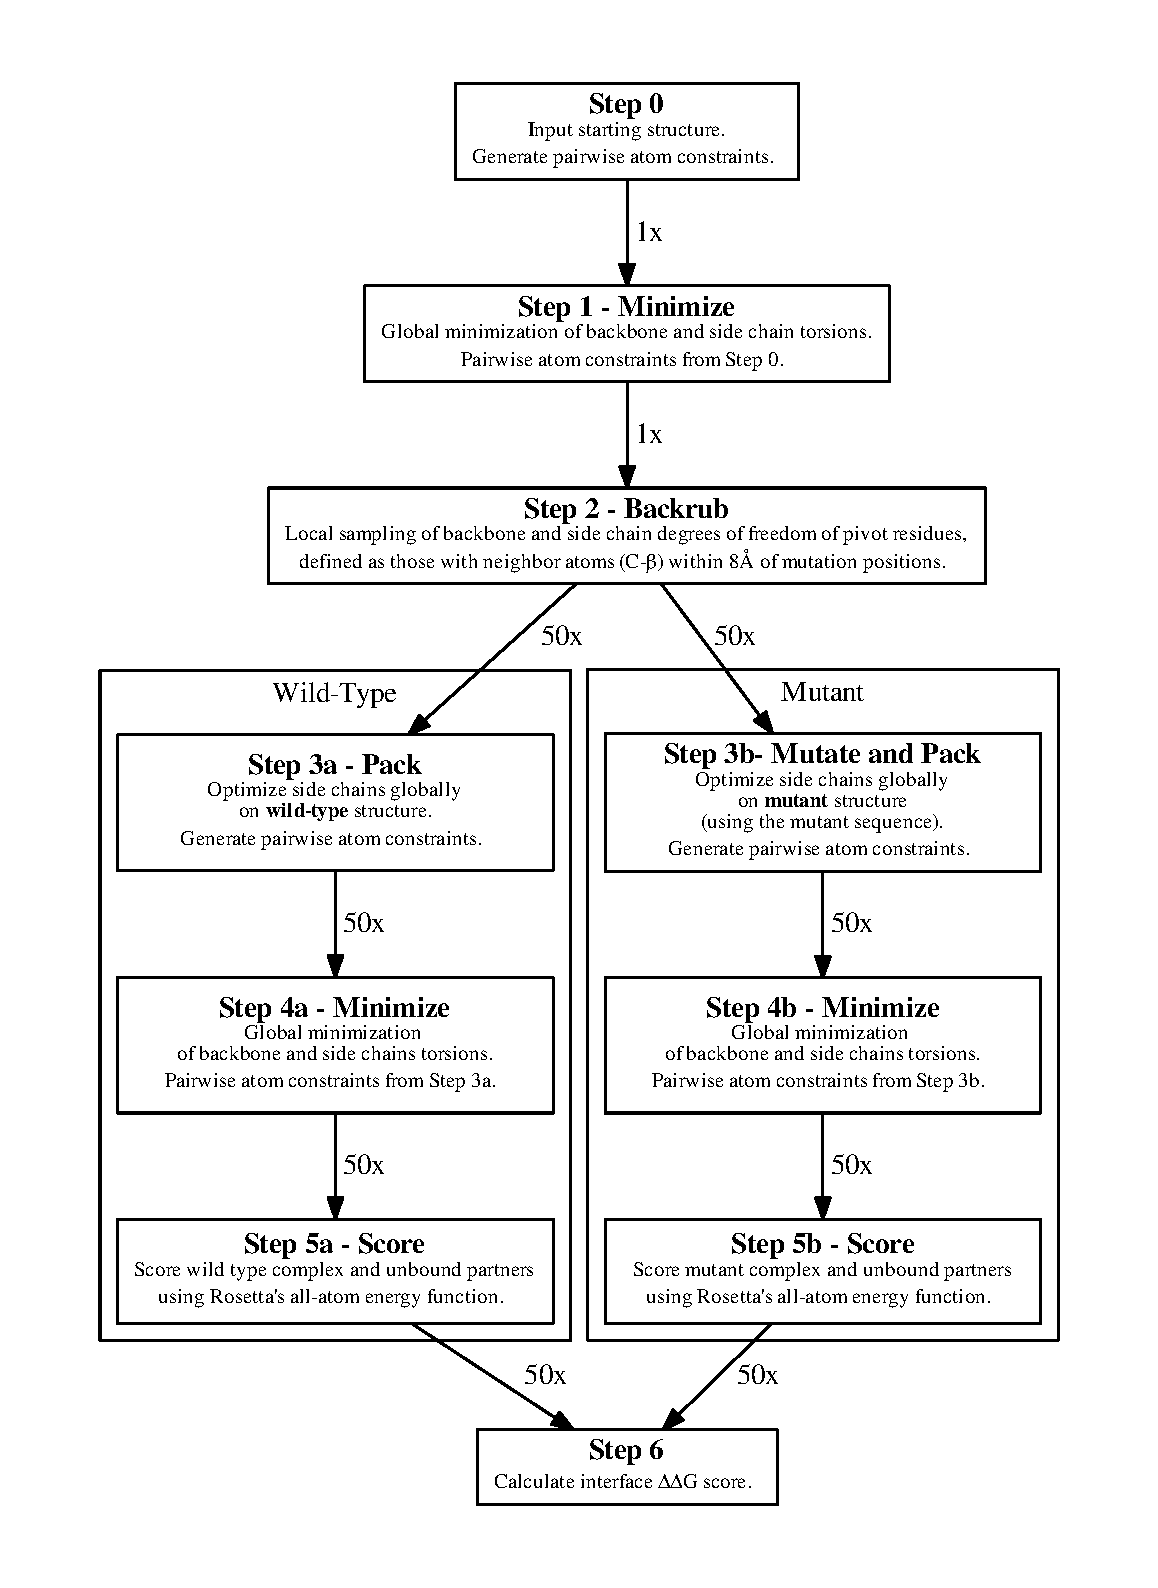
\includegraphics[width=\textwidth,keepaspectratio]{figures/fig-overview.pdf}
    \caption{
      Schematic of the flex ddG protocol method.
  } \label{fig:figure-overview}
\end{figure}

Flex ddG method steps are outlined in \cref{fig:figure-overview}. Step 1: The protocol begins with an initial minimization to calibrate the input model to the Rosetta energy function. This (and later) minimizations are performed with constraints that harmonically restrain pairwise atom distance to their values in the input crystal structure. Step 2: The backrub method is run, at a temperature of 1.2, and for up to 60,000 trials. 50 output structures are generated, which will be used as the base of conformational diversity for the rest of the week. Step 3A: For each of the 50 structure models in the ensemble (output by backrub), the Rosetta ``packer'' is run to search side chain space through the Dunbrack rotamer library built into Rosetta\cite{shapovalov_smoothed_2011}, optimizing side chains for the wild type sequence. Step 3B: Independently and in parallel to step 3A, the packer is run on the 50 backrub models, optimizing side chains for the mutant sequence. Step 4A: Minimization of each of the 50 wild-type structures, again adding pairwise atom-atom constraints to the input structure. Step 4B: Minimization of each of the 50 mutant structures. Step 5A: Each of the 50 minimized wild-type structures are scored in complex, and the individual complex components are scored individually. Step 5B: Each of the 50 minimized mutant structures are scored in complex, and the individual complex components are scored individually. Step 6: The interface ddG score is produced via Eq.~\ref{eqn:split-ddg}:

\begin{equation}\label{eqn:split-ddg}
  \begin{split}
    {\Delta\Delta}G_{bind} & ={\Delta}G^{MUT}_{bind} - {\Delta}G^{WT}_{bind}\\
    & =({\Delta}G^{MUT}_{complex} - {\Delta}G^{MUT}_{partner A} - {\Delta}G^{MUT}_{partner B})\\
    & \quad - ({\Delta}G^{WT}_{complex} - {\Delta}G^{WT}_{partner A} - {\Delta}G^{WT}_{partner B})\\
  \end{split}
\end{equation}

We evaluate performance of the protocol by comparing predicted ddG scores to known experimental values, using Pearson's correlation R, MAE, and Fraction Correct (FC). Fraction Correct is defined as the number of mutations categorized as stabilizing, neutral, or destabilizing correctly, divided by the total number of mutations in the benchmark set. Stabilizing mutations are defined as those with a ddG <= -1.0 kcal/mol, neutral as those with -1.0 kcal/mol < ddG < 1.0 kcal/mol, and destabilizing as those with ddG >= 1.0 kcal/mol.

MAE (Mean Absolute Error) is defined in Eq.~\ref{eqn:mae} as:

\begin{equation}\label{eqn:mae}
  MAE = \dfrac{1}{n}\sum\limits_{i=1}^n|y_i-x_i| = \dfrac{1}{n}\sum\limits_{i=1}^n|e_i|
\end{equation}

where $y_i$ are the predicted \ddg\ values, $x_i$ are the known, experimentally determined values, and $e_i$ is the prediction error.

\section{Results and discussion}

\subimport*{figs-and-tables/}{table-main}

Main performance of the protocol is summarized in \cref{tab:table-main}. Performance is shown for 4 prediction methods: (a) our flex ddG, backrub ensemble method, (b) the prior state-of-the-art Rosetta methodology, ddg\_monomer \cite{kellogg_role_2011}, (c) a control version of our flex ddG protocol which omits the backrub ensemble generation step, leaving only the minimization and packing steps, and (d) the ZEMu (zone equilibration of mutants) method\cite{dourado_multiscale_2014}.

Our flex ddG method outperforms the comparison methods on the complete dataset in each of the correlation, MAE, and fraction correct methods. On the small-to-large subset of mutations where we expect to see the largest performance gains from using a backbone ensemble method, we see a substantial improvement in performance as compared to the alternative methods. Performance of the flex ddG on the subset of single mutations to alanine, for which we do not expect to require intensive backbone sampling, as mutations to alanine can accommodate much of ramachandran space\cite{cunningham_high-resolution_1989}, also is competitive or outperforms the alternative methods. Finally, our method shows improved performance compared to the control method and ddg\_monomer on the subset of multiple mutations, but does not match the performance of the ZEMu method.
However, flex-ddG outperforms ZEMu on multiple mutations if none of the mutations are to alanine (\cref{tab:table-mult}).

The underlying scatterplots for the flex ddG and control methods on the complete dataset and small-to-large subsets are shown in \cref{fig:figure-scatter}. Scatterplots for the underlying data behind the rest of the rows in \cref{tab:table-main} is shown in the Supplementary Information.

\subimport*{figs-and-tables/}{figure-scatter}

\subimport*{figs-and-tables/}{structs-v-corr-WildTypeComplex-zemu-12-60000-rscript-validated-t14}

\subsection{Effect of averaging more structures}

\cref{fig:structs-v-corr-WildTypeComplex-zemu-12-60000-rscript-validated-t14} shows the effect on performance as scores from an increasing number of structures are averaged.
The structures used are first sorted by the score of the score of the corresponding repacked and minimized wild type structure.
\cref{fig:structs-v-corr-WildTypeComplex-zemu-12-60000-rscript-validated-t14}(a) shows perfomance on the complete dataset.
As more structures, of increasingly high wild type complex score, are averaged, correlation with known experimental values increases.
Conversely, performance for the no backrub control method (shown in light blue) decreases as more structures are average.
This result indicates that sampling with backrub adds information that improves ddG calculation, and adds it in such a way that cannot be quantified through score alone, as the additional structures being averaged have higher scores \cref{fig:wildtypecomplex-scores-complete}, and would traditionally be though of as being less predictive.

The ddg\_monomer method also sees an increase in performance on the complete dataset as more structures are averaged (\cref{fig:structs-v-corr-WildTypeComplex-ddg-monomer-16-003-zemu-2}), indicating that ramping the repulsive term of the energy function during minimization in ddg\_monomer also improves results by sampling conformational space more broadly.

Averaging across more structures show an even stronger positive effect on correlation \cref{fig:structs-v-corr-WildTypeComplex-zemu-12-60000-rscript-validated-t14}(b) for the subset of small-to-large mutations.
However, the subset of multiple mutations (where none are mutations to alanine) shown in \cref{fig:structs-v-corr-WildTypeComplex-zemu-12-60000-rscript-validated-t14}(c) does not see monotonically increasing performance as more structures are averaged, indicating that more parameterization of the backrub method might be necessary for multiple mutations.

The improved performance effect is also present in \cref{fig:structs-v-corr-WildTypeComplex-zemu-12-60000-rscript-validated-t14}(d) for the subset of single mutations to alanines, a subset where it is not expected that increased sampling is neccessary, indicating that increased sampling at least does not hurt in this case.

As it is not possible to select 20 best-scoring structures without generating a full ensemble of 50, and as the performance when choosing structures sorted in this fashion is not significantly improved over the results in \cref{fig:structs-v-corr-id-zemu-12-60000-rscript-validated-t14} (where there is no sorting), simply generating 20-30 structures should constitute sufficient sampling for most use cases.

\subsection{Effect of changing backrub temperature}

Sampling is also controlled by changing how many steps the backrub simulation runs for.
\cref{fig:steps-v-corr} shows the performance effect of increasing backrub simulation length (while averaging all 50 structures at each output step).
Increased performance is not simply a result of scores decreasing as the simulation progresses, as the score of the minimized wild type complex does not decrease uniformly across the sampled ensemble as the simulation progresses (\cref{fig:wildtypecomplex-scores-complete}).

When viewing the effect on sampling on increases steps (vs. previously increasing number of structures), we see relatively flat performance on the complete dataset and subset of single mutations to alanine.
As with increasing number of structures, we also see increased performance on the subset of small-to-large mutations.
Unlike when increasing the number of averaged structures, we see improved performance with additional sampling (from longer backrub simulations) on the subset of multiple mutations (not to alanine). This indicates that the effects of increasing sampling through creating more structure models and running longer backrub simulations are not equivalent, and that both sampling parameters are important to consider when running the flex ddG protocol.

\subsection{Score analysis}

We applied machine learning to our cases to try and study which individual score terms were informative.
GAM (generalized additive model) \cite{wood_fast_2011}.

\subsection{Structure analysis}

As mean backrub ensemble RMSD increases (\cref{fig:t14-mean-ensemble-error}), we don't see any significant correlation between mean ensemble RMSD and ddG error (\cref{fig:spear-corr-rmsd-error}). E.g. we can't measure that we are sampling more effectively through mean ensemble RMSD.

\section{Conclusions}

We have made sampling better, maybe it is time to also make scoring better. REF energy energy does not improve performation (\cref{tab:table-ref}).
GAM reweighting indicates potential future benefits of non-linear reweighting of Rosetta energy function terms, particularly in this case of interfaces.

Not changing the unbound models might work because it adds noise, and because the mobility of amino acids at the dimeric interface is generally lower than for other amino acids at the protein surface \cite{zen_comparing_2010}.

\subsection{unfinished}

Why do our backrub ensembles work better than \cite{kamisetty_accounting_2011} and \cite{kellogg_role_2011}, which also used backrub exactly (GOBLIN) or something like it (Kellogg). Where the sampling takes place, and how much, are important. We've focused around mutations.

Why no boltzmann weighting? If we are sampling the underlying distribution unbiased, we wouldn't need to.

Entropy.

\begin{itemize}
\item Monomeric Rosetta ddG does not work for interfaces
\item As stated in intro, ensembles have advantages, etc.
\item Dataset: zemu (why better than skempi). Table 1
\item General prediction protocol in figure 1
\item Metric description: pearson’s R, fraction correct, MAE
\item Description of main results, subsets, and comparison to zemu method
\item Scatter plots and table
\item Number of structures in ensemble average, discuss filtering structures by score (ref supp. fig). Fig 4 - one panel showing number of structures effect on correlation (at best backrub step)
\item Structure comparison - RMSD deviation are subtle. Torsions could be more informative?
\item We applied machine learning to our cases to try and study which individual score terms were informative
\end{itemize}

\subsection{more unfinished}
Local conformational sampling

Perhaps because
As the protein folding funnel is narrower near the free energy minimum {Dill, From Levinthal to pathways to funnels (include this?)}, it should be more possible to find a discrete number of states to represent in an ensemble and use in ddG modeling,
We can capture the thin part of the funnel:
“backrub sampling may capture a sizable fraction of localized conformational changes that occur in proteins” \cite{humphris_prediction_2008}

Questions:
Shouldn’t it be easier to predict interface ddGs, as we don’t need to consider the stability effects of mutants in the unfolded state
